When charged particles interact with matter, only the electromagnetic force is of importance. The
following reactions lead to loss of energy of the charged particles:

\begin{itemize}
  \item ionisation of the atoms in the detector
  \item excitation of the atoms in the detector
  \item bremsstrahlung (relevant for electrons/positrons)
  \item \v{C}erenkov radiation
  \item transition radiation
\end{itemize}

\[-\left(\frac{dE}{dx}\right)_{\text{tot}} = -\left(\frac{dE}{dx}\right)_{\text{coll}}
-\left(\frac{dE}{dx}\right)_{\text{rad}} -\left(\frac{dE}{dx}\right)_{\text{pair}}
-\left(\frac{dE}{dx}\right)_{\text{photo}} -\left(\frac{dE}{dx}\right)_{\text{compton}}
-\left(\frac{dE}{dx}\right)_{\text{kal}}\]

As an example, the total loss of energy $-\frac{dE}{dx}$ of muons in copper is shown in fig.
\ref{enenergylossInCopper}. Most of it can be described by the Bethe formula (the derivation is
explained in the next chapter). Different energies of the projectiles leads through different
interaction to loss of energy.

\begin{figure}[H]
	\centering
	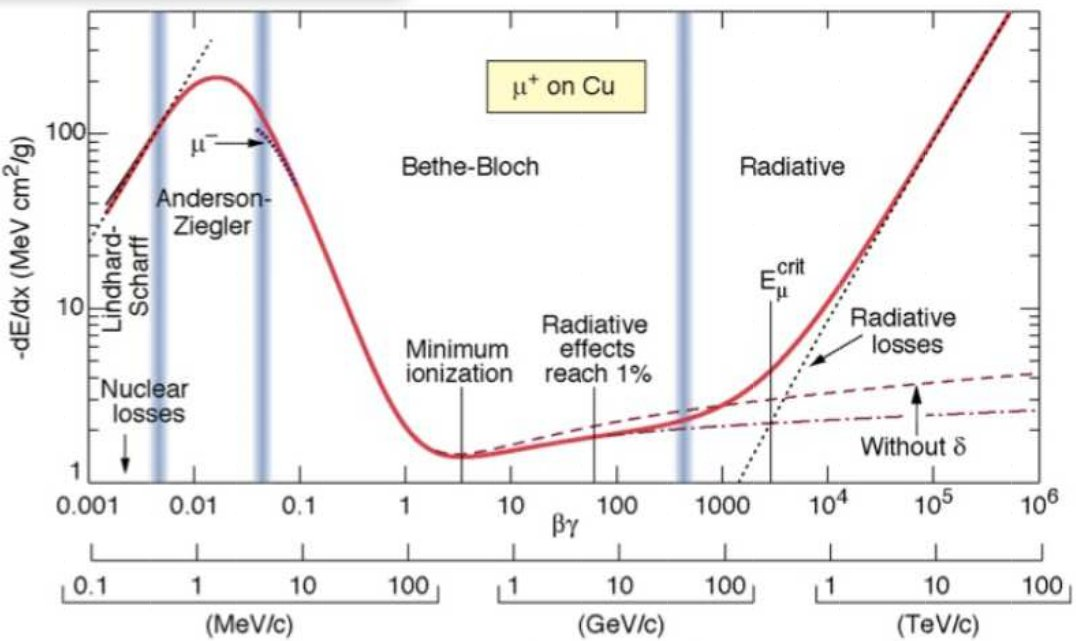
\includegraphics[width=0.5\textwidth]{bethebloch.jpg}
	\caption{Total loss of energy of muons in copper}
	\label{enenergylossInCopper}
\end{figure}

\begin{figure}[H]
	\centering
	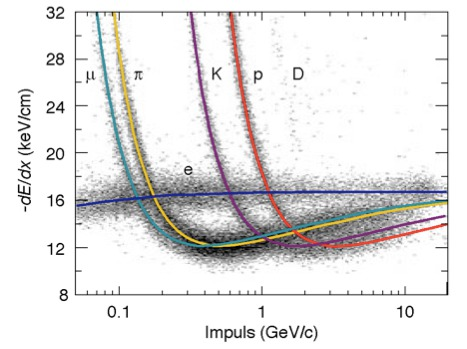
\includegraphics[width=0.5\textwidth]{bethebloch2.jpg}
	\caption{$\frac{dE}{dx}$-Kurven für verschiedene Teilchen (gemessen in der
	PEP4/9-TPC)}
	\label{}
\end{figure}

Notice: $\frac{dE}{dx}$ for heavy particles (e.g. $\alpha$ particles) corresponds well to the Bethe
formula. The energy loss caused by ionisation or excitation of target electrons is dominant.
$\frac{dE}{dx}$ for electrons/positrons, however, do not obey the Bethe formula.
